\documentclass{beamer}
\mode<presentation>{}
\usefonttheme{professionalfonts}

\usepackage[T1]{fontenc}
\usepackage{libertine}
\renewcommand*\ttdefault{txtt}

\usepackage{algorithm}
\usepackage{algpseudocode}
\usepackage{array}
\usepackage{caption}
\usepackage{graphicx}
\usepackage{mathtools}
\usepackage{rnamacros}
\usepackage{textcomp}
\usepackage{xspace}

\graphicspath{ {images/} }

\newcommand{\pryme}{\textquotesingle\xspace}

\title[RNA Thermodynamics with the FFT]{On the use of polynomial interpolation to improve the performance of dynamic programming algorithms with discrete distance metrics}
\author{Evan Senter}
\date{2015}

\AtBeginSection[]
{
  \begin{frame}<beamer>{Outline}
    \tableofcontents[currentsection]
  \end{frame}
}

\begin{document}

\frame{\titlepage}

% \begin{frame}
%   \frametitle{}
%   \begin{block}{}
%   \begin{itemize}
%   \item
%   \end{itemize}
%   \end{block}
% \end{frame}

\section{Motivation}

\begin{frame}
  \frametitle{Goal of Presentation}
  \begin{block}{Structure of talk}
  \begin{itemize}
  \item Provide motivation for synthetic RNA design
  \item Overview of thermodynamic-based computational analysis
  \item Describe algorithm to generate a discretized, coarse-grained energy landscape
  \item Show how polynomial interpolation improves asymptotics
  \item Highlight practical applications of energy landscapes
  \end{itemize}
  \end{block}
\end{frame}

\begin{frame}
  \frametitle{Why RNA?}
  \begin{itemize}
  \item The central dogma of DNA is a lie
  \item RNA has been shown to regulate many aspects of the cellular machinery
  \item What was once considered `junk DNA' is now appreciated as non-coding RNA `ncRNA'
  \end{itemize}
\end{frame}

\begin{frame}
  \frametitle{Why RNA?}
  \begin{itemize}
  \item RNA is an enzymatically active molecule (hydroxyl group on 2\pryme carbon is highly reactive)
  \item Secondary structure is more mathematically tractable than proteins
  \item Interesting applications of {\em cis}-regulation via motifs in the 5\pryme untranslated region of coding RNAs
  \end{itemize}
\end{frame}

\section{Computational RNA background}

\begin{frame}
  \frametitle{RNA Representation}
  \begin{block}{Sequence}
  An RNA sequence is a string $\seq = \seqN$, where $s_i \in \{\text{A,\,U,\,G,\,C}\}$
  \end{block}
  \begin{block}{Structure}
  An secondary structure \str compatible with \seq is a collection of base pair tuples such $(i,j)$, such that:
  \begin{itemize}
  \item $(\seq_i, \seq_j) \in \bpSet$
  \item $1 \le i \le i+\theta < j \le n$ where $\theta \ge 0$
  \item Given $(i,j), (x,y)$ from \str, $i=x \iff j=y$
  \item Given $(i,j), (x,y)$ from \str, $i<x<j \iff i<y<j$
  \end{itemize}
  \end{block}

  \begin{align*}
    \bpSet =
  \{\text{(A,\,U),\,(U,\,A),\,(G,\,C),\,(C,\,G),\,(G,\,U),\,(U,\,G)}\}
  \end{align*}
\end{frame}

\begin{frame}
  \frametitle{Structural Motifs}
  \begin{columns}
  \column{.6\textwidth}
  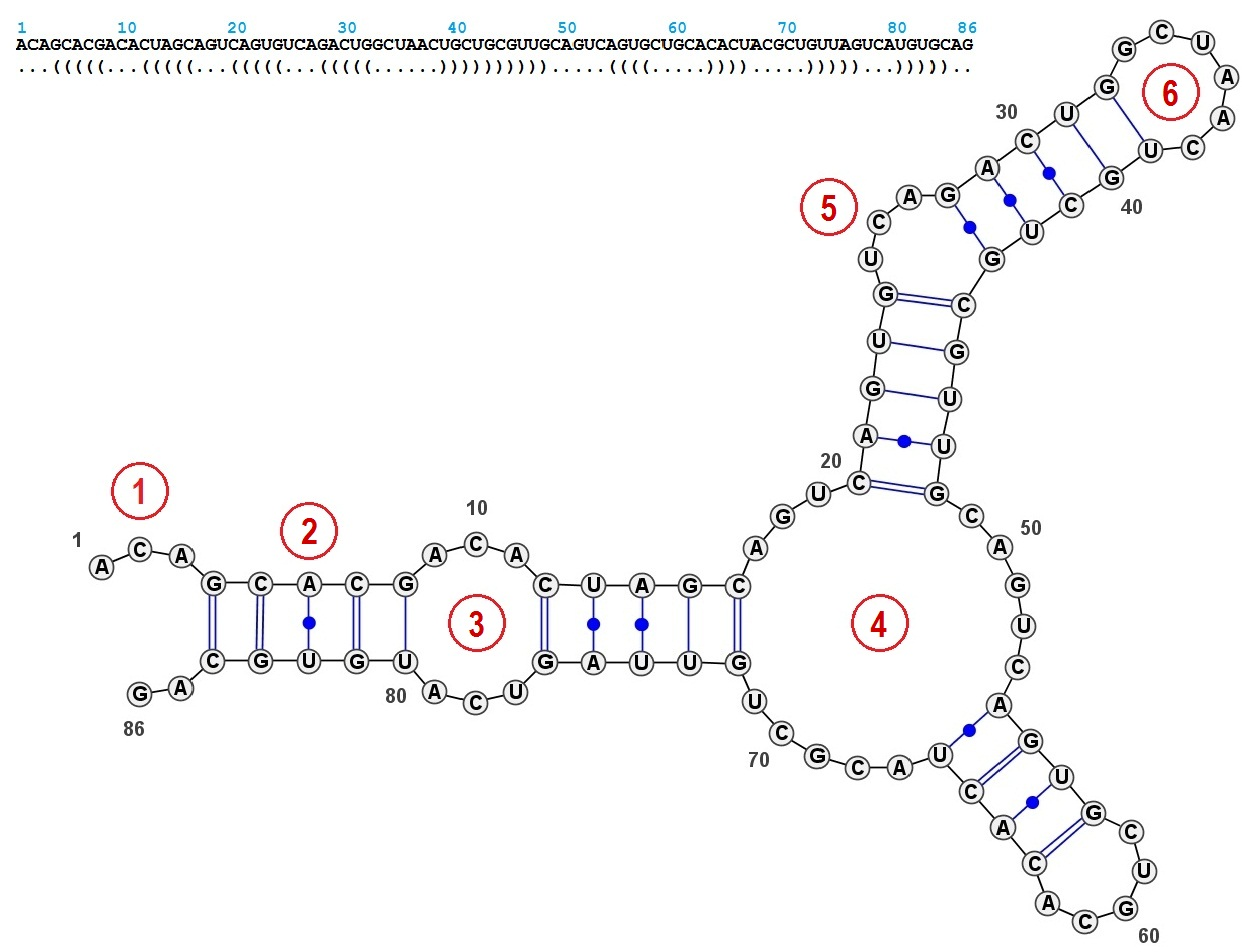
\includegraphics[width=.9\linewidth]{rnass}

  \column{.4\textwidth}
  \begin{block}{Structural Motifs}
  \begin{enumerate}
  \item Exterior loop
  \item Stack
  \item Interior loop
  \item Multiloop
  \item Bulge
  \item Hairpin
  \end{enumerate}
  \end{block}
\end{columns}
\end{frame}

\begin{frame}[fragile]
  \frametitle{RNA Notation}
  \begin{block}{Yeast tRNA\textsuperscript{phe} dot-bracket notation}
  \scriptsize\begin{semiverbatim}
  GCGGAUUUAGCUCAGUUGGGAGAGCGCCAGACUGAAGAUCUGGAGGUCCUGUGUUCGAUCCACAGAAUUCGCACCA
  (((((((..((((........)))).(((((.......))))).....(((((.......))))))))))))....
  \end{semiverbatim}
  \end{block}

  \begin{block}{Yeast tRNA\textsuperscript{phe} structural diagram}
  \vspace{1ex}
  \centering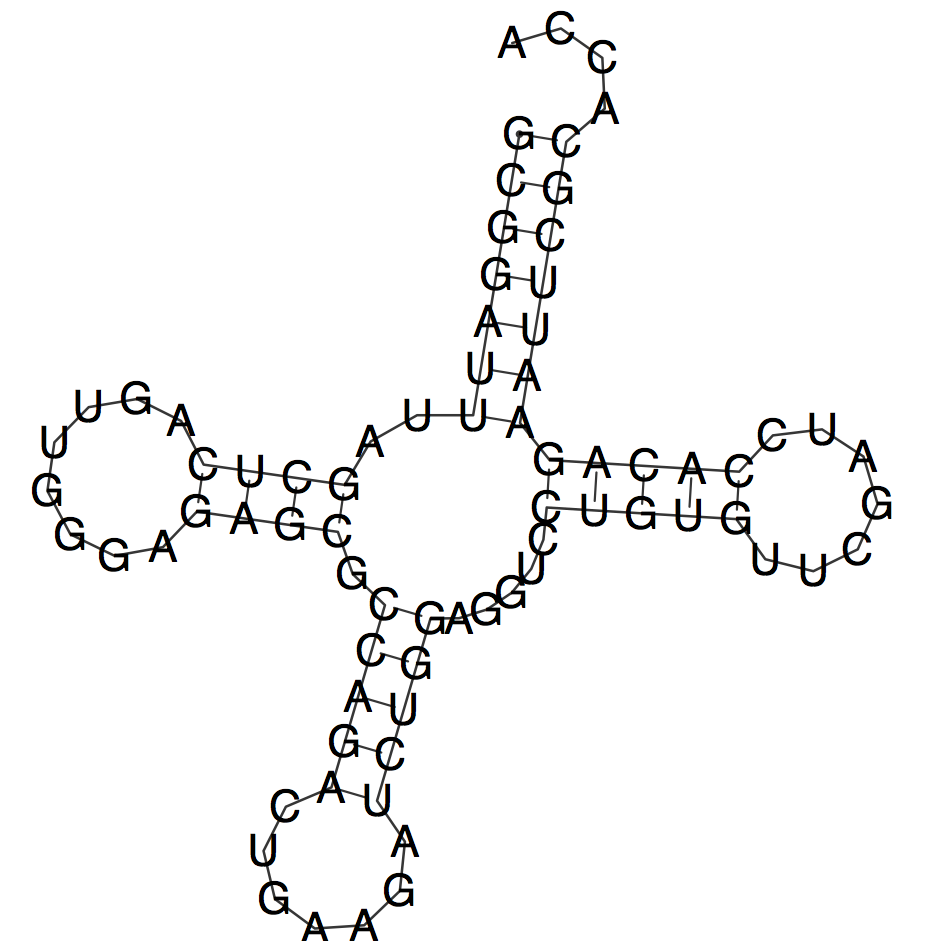
\includegraphics[scale=.25]{rna.png}
  \end{block}
\end{frame}

\section{Problem definition}

\begin{frame}
  \frametitle{Problem Definition}
  \begin{block}{Desire}
  Given an input sequence \seq and two input structures \strA, \strB, we would like to compute \alert{all} possible structures \strS compatible with \seq, and bin them into discrete sets based on their {\em distance} to \strA and \strB
  \end{block}

  \begin{alertblock}{Issue}
  Consider $\mathbb{S}$ to be the set of all structures compatible with \seq. It has been shown that $|\mathbb{S}|$ grows exponentially with sequence length $n$
  \end{alertblock}

  \begin{block}{Refinement}
  Rather than store $\mathbb{S}$ at any point in time, we will use dynamic programming to compute the thermodynamic properties of these bins
  \end{block}
\end{frame}

\begin{frame}[fragile]
  \frametitle{Concrete Example}
  \begin{columns}[t]
  \column{.25\textwidth}
  \begin{block}{Input}
  \vspace{1em}
  \ms{GGAAACC} $= \seq$  \\
  \ms{.......} $= \strA$ \\
  \ms{.(...).} $= \strB$
  \end{block}

  \column{.37\textwidth}
  \begin{block}{Structures}
  \vspace{1em}
  \ms{.......}\;$0.00 \frac{\text{kcal}}{\text{mol}}, \alert{[0, 1]}$
  \ms{.(...).}\;$4.40 \frac{\text{kcal}}{\text{mol}}, \alert{[1, 0]}$
  \ms{(....).}\;$2.30 \frac{\text{kcal}}{\text{mol}}, \alert{[1, 2]}$
  \ms{.(....)}\;$4.10 \frac{\text{kcal}}{\text{mol}}, \alert{[1, 2]}$
  \ms{(.....)}\;$4.20 \frac{\text{kcal}}{\text{mol}}, \alert{[1, 2]}$
  \ms{((...))}\;$2.10 \frac{\text{kcal}}{\text{mol}}, \alert{[2, 1]}$
  \end{block}

  \column{.38\textwidth}
  \begin{block}{Output}
  \begin{align*}
  \begin{bmatrix}
  0 & \alert{0.9595} & 0 \\
  \alert{0.0001} & 0 & \alert{0.0086} \\
  0 & \alert{0.0318} & 0
  \end{bmatrix}
  \end{align*}
  \end{block}
  \end{columns}
\end{frame}

\begin{frame}
  \frametitle{Concrete Example}
  \begin{block}{Energy landscape between two metastable structures of {\em L.collosoma} spliced leader RNA}
  \vspace{1em}
  \centering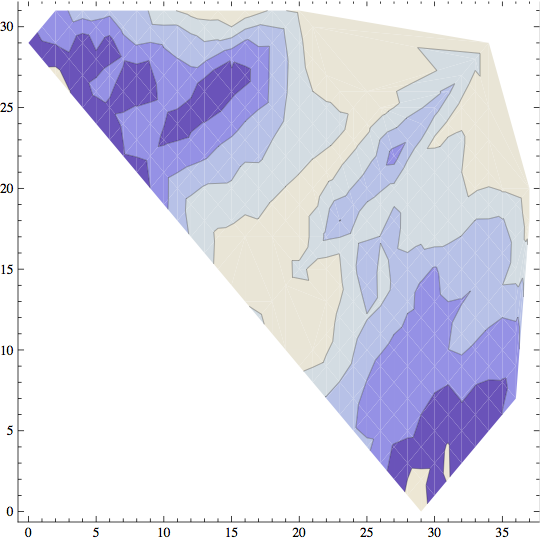
\includegraphics[scale=.5]{2dgrid.png}
  \end{block}
\end{frame}

\begin{frame}
  \frametitle{Base Pair Distance}
  \begin{block}{Symmetric distance}
  \begin{align*}
    \dBP{\str}{\strT} = |\str \cup \strT| - |\str \cap \strT|
  \end{align*}
  \end{block}

  \begin{block}{Distance between two structures}
  \begin{align*}
  \begin{split}
    \dBP{\str_{[i,j]}}{\strT_{[i,j]}} &=
  |\{ (x,y): i \leq x<y\leq j, \\
  & (x,y) \in \str - \strT \text{ or } (x,y) \in \strT - \str \}| = k
  \end{split}
  \end{align*}
  \end{block}
\end{frame}

\begin{frame}
  \frametitle{Parameterized Partition Function, 1D}
  \begin{block}{\bfZ{}{} binned by $k$}
  \begin{align*}
  \bfZ{k}{} = \bfZ{k}{1,n} =
  \sum_{\mathclap{\substack{\str \text{ such that }\rule[-.5ex]{0pt}{0pt} \\ \dBP{\str}{\strSt}=k}}}\;
  \boltzF{\str}
  \end{align*}
  \end{block}
\end{frame}

\begin{frame}
  \frametitle{Recursions to compute \bfZ{k}{i,j}}
  \begin{block}{Structural decomposition from one target}
  \begin{align*}
    \bfZ{k}{i,j} = \bfZ{k-b_0}{i,j-1}\enspace +
  \sum_{\substack{s_r s_j \in \bpSet, \\ i \le r<j}}
  \left(
  \boltzNuss{r,j}\enspace \sum_{\mathclap{w+w'=k-b(r)}}\quad
  \bfZ{w}{i,r-1} \bfZ{w'}{r+1,j-1}
  \right)
  \end{align*}
  \end{block}
\end{frame}

\begin{frame}
  \frametitle{Parameterized Partition Function, 2D}
  \begin{block}{\bfZ{}{} binned by $x,y$ pairs}
  \begin{align*}
  \bfZ{x,y}{1,n}\;=\;
  \sum_{\mathclap{\substack{
  \str \text{ such that } \rule[-.5ex]{0pt}{0pt} \\
  \dBP{\str}{\strA} = x,\,\dBP{\str}{\strB} = y}}}\enspace
  \boltzF{\str}
  \end{align*}
  \end{block}
\end{frame}

\begin{frame}
  \frametitle{Recursions to compute \bfZ{x,y}{i,j}}
  \begin{block}{Structural decomposition from two targets}
  \begin{align*}
    \begin{split}
  & \bfZ{x,y}{i,j} = \bfZ{x- \omega_0,y-\beta_0}{i,j-1}\enspace + \\
  & \sum_{\substack{s_k s_j \in \bpSet, \\ i \le k<j}}
  \left(
  \boltzNuss{k,j}\quad
  \sum_{\mathclap{u+u'=x- \omega(k)}}\hspace{3.75em}
  \sum_{\mathclap{v+v'=y-\beta(k)}}\quad
  \bfZ{u,v}{i,k-1} \cdot \bfZ{u',v'}{k+1,j-1}
  \right)
  \end{split}
  \end{align*}
  \end{block}
\end{frame}

\begin{frame}
  \frametitle{Partition function of a variable $x$}
  \begin{block}{Only compute \emZ{i,j}{x} instead of \bfZ{x,y}{i,j}}
  \begin{align*}
    \begin{split}
  & \emZ{i,j} = \emZof{i,j-1}{x} \cdot x^{ \omega_0n+\beta_0} + \\
  &\sum_{\substack{s_k s_j \in \bpSet,\\i\le k<j}}
  \left(e^{\frac{-E_0(k,j)}{RT}}\cdot
  \emZof{i,k-1}{x} \cdot \emZof{k+1,j-1}{x}\cdot x^{ \omega(k)n+\beta(k)} \right)
  \end{split}
  \end{align*}
  \end{block}
\end{frame}

\section{Optimization using Fast Fourier Transform}

\begin{frame}
  \frametitle{FFT background}
  \begin{block}{Complex {\em k}th roots of unity}
  \begin{align*}
   \omega_0=\exp(\frac{0\cdot 2\pi i}{n^2}), \omega_1=\exp(\frac{1\cdot 2\pi i}{n^2}),\dots, \omega_{n^2-1}=\exp(\frac{(n^2-1)\cdot 2\pi i}{n^2})
  \end{align*}
  \end{block}

  \begin{block}{Evaluate \emZ{i,j}{x} for all $n^2$ roots of unity}
  \begin{align*}
  y_0=\emZof{}{ \omega_0},\dots,y_{n^2-1}=\emZof{}{ \omega_{n^2-1}})
  \end{align*}
  \end{block}

  \begin{block}{Represent results of evaluation in column form}
  \begin{align*}
    \bfY = (y_0,\dots,y_{n^2-1})^{\text T}
  \end{align*}
  \end{block}
\end{frame}

\begin{frame}
  \frametitle{Vandermonde matrix}
  \begin{block}{Matrix construction}
  \begin{align*}
    V_{n} =
  \left(
  \begin{array}{rrrrr}
  1 & 1 & 1 & \dots & 1 \\
  1 & \omega & \omega^2 & \dots & \omega^{n-1} \\
  1 & \omega^2 & \omega^4 & \dots & \omega^{2(n-1)} \\
  1 & \omega^3 & \omega^6 & \dots & \omega^{3(n-1)} \\
  \vdots & \vdots & \vdots & \vdots & \vdots \\
  1 & \omega^{n-1} & \omega^{2(n-1)} & \dots & \omega^{(n-1)(n-1)} \\
  \end{array}
  \right)
  \end{align*}
  \end{block}
\end{frame}

\begin{frame}
  \begin{definition}
  Define the FFT to be the $O(n \log n)$
  algorithm to compute the Discrete Fourier Transform (DFT), defined
  as the matrix product $\bfY = V_{n} {\bf A}$
  \end{definition}

  \begin{align*}
  \left(
  \begin{array}{l}
  y_0 \\
  y_1 \\
  y_2 \\
  \vdots \\
  y_{n^2-1} \\
  \end{array}
  \right)
  = V_n \cdot
  \left(
  \begin{array}{l}
  a_0 \\
  a_1 \\
  a_2 \\
  \vdots \\
  a_{n^2-1} \\
  \end{array}
  \right)
  \end{align*}
\end{frame}

\begin{frame}
  Since we defined $\bfY =
  (y_0,\dots,y_{n-1})^{\text T}$, where:

  \begin{align*}
  y_0=\emZof{}{\omega_0},\dots,y_{n^2-1}=\emZof{}{\omega{n^2-1}})
  \end{align*}

  and $\omega_k = \exp(\frac{2\pi ki}{n^2})$, it follows that the coefficients
  $c_{rn+s}=\bfZ{rn+s}{1,n}$ in the polynomial:

  \begin{align*}
  \emZ{} = c_0 + c_1 x + \dots + c_{n^2-1} x^{n^2-1}
  \end{align*}

   can be computed using the \fft, and:

  \begin{align*}
    c_{rn+s}=\;=\;
    \sum_{\mathclap{\substack{
    \str \text{ such that } \rule[-.5ex]{0pt}{0pt} \\
    \dBP{\str}{\strA} = r,\,\dBP{\str}{\strB} = s}}}\enspace
    \boltzF{\str}
  \end{align*}
\end{frame}

\section{Results}

\begin{frame}
  \frametitle{Performance Characteristics}
  \begin{columns}
  \column{.5\textwidth}
  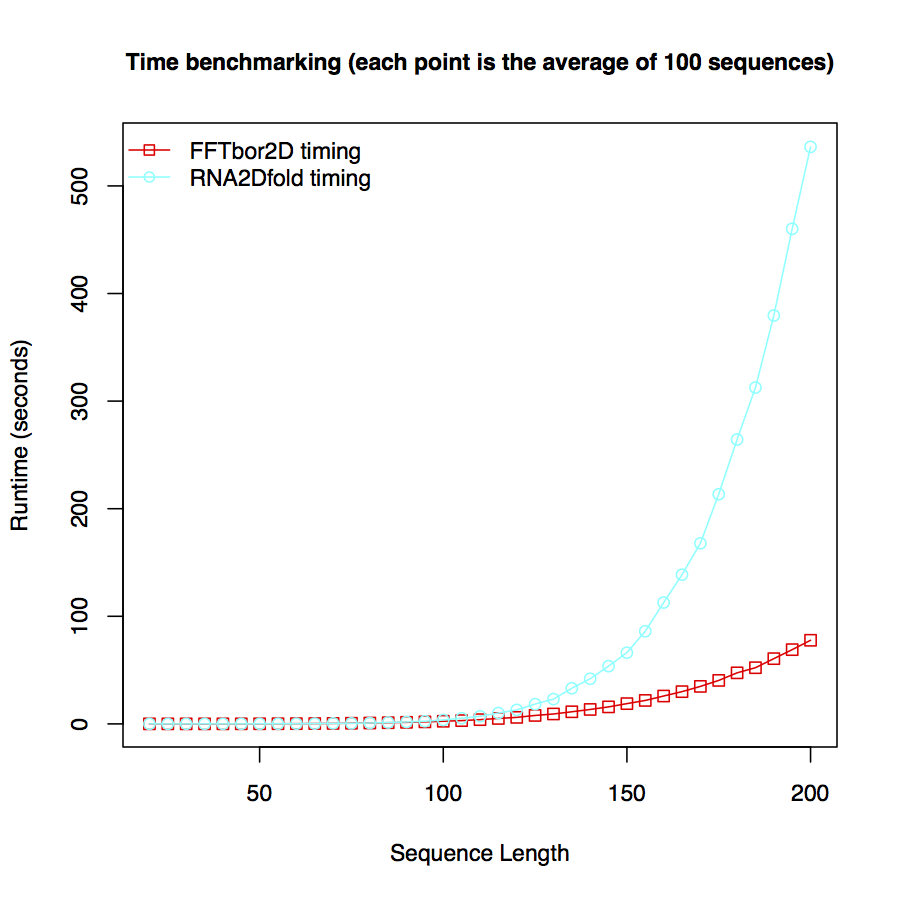
\includegraphics[width=\linewidth]{fft2dspeed.png}

  \column{.5\textwidth}
  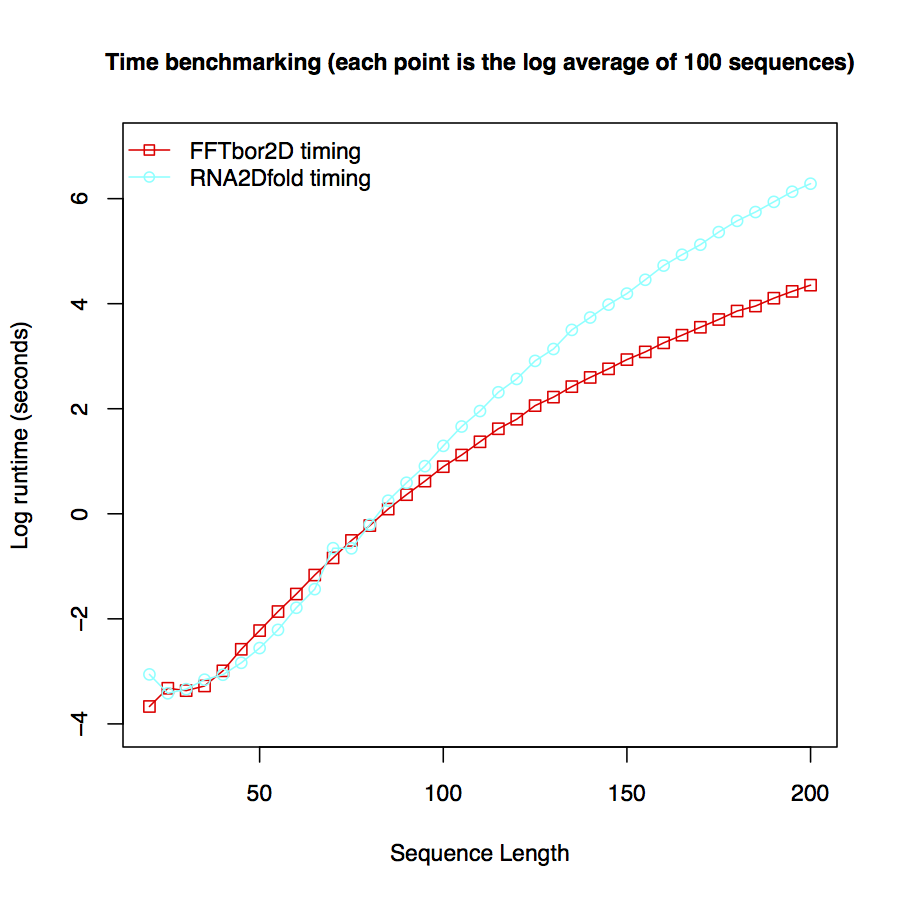
\includegraphics[width=\linewidth]{fft2dlogscale.png}

  \end{columns}
\end{frame}

\begin{frame}
  \frametitle{Performance Characteristics}
  \begin{columns}
  \column{.5\textwidth}
  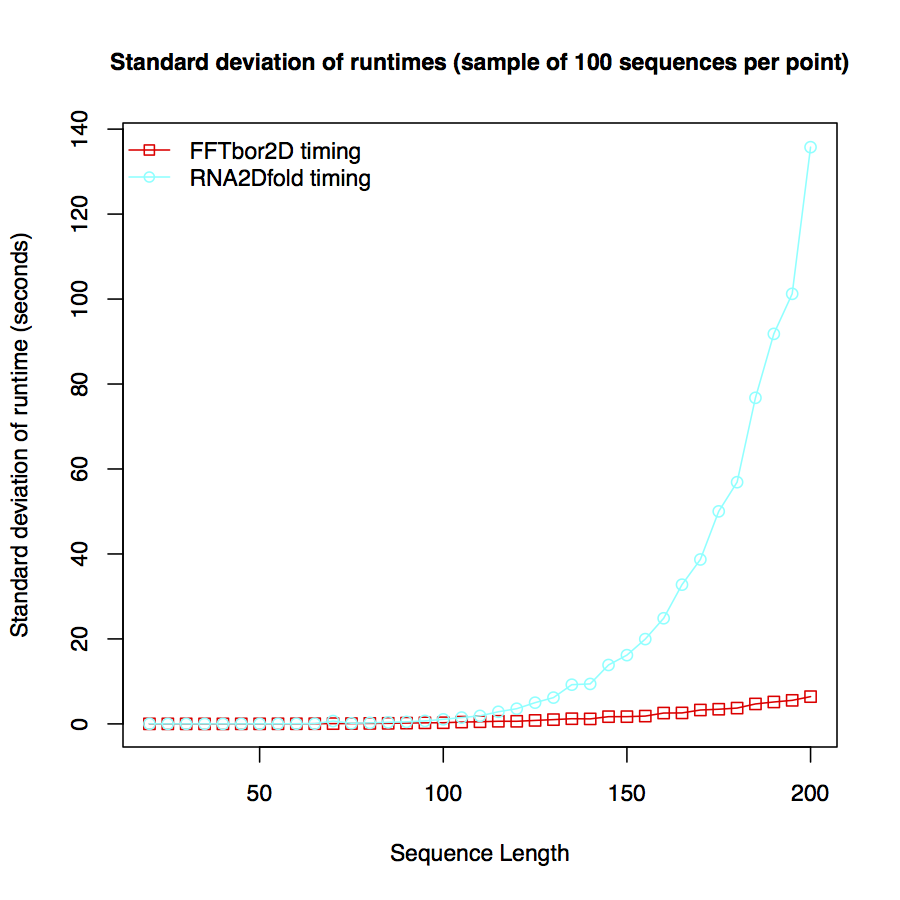
\includegraphics[width=\linewidth]{fft2dstdev.png}

  \column{.5\textwidth}
  \begin{itemize}
  \item Approach using FFT goes from \On{7} to \On{5}
  \item We observe a real performance gain in line with 100x speedup
  \item Memory requirements drop from \On{4} to \On{2}
  \item More consistent performance characteristics
  \end{itemize}
  \end{columns}
\end{frame}

\begin{frame}
  \frametitle{Questions?}

  \centering Thanks for your time!
\end{frame}

\end{document}
